\renewcommand{\thesection} {\Alph{section}}
\setcounter{section}{1}
\section{System guide}

\subsection{JavaScript library}

All of the following sources are available in the \href{https://github.com/vojto/atmos2}{GitHub repository of Atmosphere}.

\subsubsection{AppContext}

\subsubsection*{Pubic Methods}
\item
\textbf{exists}
Check if object exists.
\item
\textbf{updateOrCreate}
Updates or creates object with passed data.
\item
\textbf{create}
Creates new object.
\item
\textbf{update}
Updates object with data.
\item
\textbf{changeID}
Changes ID of an object.
\item
\textbf{relation}
Sets up relationship for an object.
\item
\textbf{objectAtURI}
Returns object at passed URI.
\item
\textbf{dataForURI}
Returns data for object at passed URI.
\item
\textbf{dataForObject}
Returns data for object.
\item
\textbf{objectURI}
Returns URI of an object.
\item
\textbf{allURIs}
Returns URIs of all objeccts.
\item
\textbf{destroy}
Destroy object.
\subsubsection*{Private Methods}
\item
\textbf{\_modelForURI}
Returns model for URI.

\subsubsection{MessageClient}
\subsubsection*{Pubic Methods}
\item
\textbf{connect}
Connects the client.
\item
\textbf{close}
Closes the connection.
\item
\textbf{socketDidClose}
Callback called when socket closes.
\item
\textbf{send}
Sends a message.
\item
\textbf{parseNotification}
Parses incoming notification.
\item
\textbf{parseUpdate}
Parses incoming update notification

\subsubsection{MetaContext}
\subsubsection*{Pubic Methods}
\item
\textbf{configure}
Configures meta context.
\item
\textbf{markURIChanged}
Marks object at URI as changed.
\item
\textbf{findOrCreateObjectAtURI}
Finds or creates meta object for URI.
\item
\textbf{objectAtURI}
Returns meta object for URI.
\item
\textbf{createObjectAtURI}
Creates new meta object for URI.
\item
\textbf{saveObject}
Saves meta object.
\item
\textbf{deleteObject}
Deletes meta object.
\item
\textbf{changeIDAtURI}
Changes ID of meta object for URI.
\item
\textbf{isURILocalOnly}
Returns true if object at URI has flag of being local only.
\item
\textbf{isURIChanged}
Returns true if object at URI has flag of being changed.
\item
\textbf{changedObjects}
Returns all changed objects.
\item
\textbf{markURISynced}
Marks object at URI as synced. (Removes the flag of being changed.)

\subsubsection{ResourceClient}
\subsubsection*{Pubic Methods}
\item
\textbf{fetch}
Fetches remote items.
\item
\textbf{updateFromItems}
Updates local storage from remote JSON object.
\item
\textbf{updateFromItem}
Updates local object from remote JSON object.
\item
\textbf{itemsFromResult}
Extracts items from JSON result.
\item
\textbf{save}
Saves object remotely.
\item
\textbf{execute}
Executes requests against remote service.
\item
\textbf{request}
Creates remote request.
\item
\textbf{ajax}
Makes AJAX call.
\item
\textbf{addHeader}
Adds header to be sent with every HTTP request.

\subsubsection*{Private Methods}
\item
\textbf{\_updateFromData}
Updates local object from data.
\item
\textbf{\_removeObjectsNotInList}
Removes local objects that were not included in the response.
\item
\textbf{\_findPathForObject}
Returns remote path for local object.
\item
\textbf{\_findPathForURI}
Returns remote path for object with URI.
\item
\textbf{\_findPath}
Finds path using routing table.

\subsubsection{Synchronizer}
\subsubsection*{Pubic Methods}

\item
\textbf{constructor}
Constructs synchronizer.
\item
\textbf{bind}
Binds event.
\item
\textbf{trigger}
Triggers event.
\item
\textbf{unbind}
Unbinds event.
\item
\textbf{updateOrCreate}
Updates or create local object with data specified.
\item
\textbf{fetch}
Fetches remote object.
\item
\textbf{save}
Saves local object remotely.
\item
\textbf{execute}
Executes request.
\item
\textbf{request}
Creates request.
\item
\textbf{markObjectChanged}
Marks object as changed.
\item
\textbf{markURISynced}
Marks object as synced.
\item
\textbf{setNeedsSync}
Schedules synchronization for the next cycle.
\item
\textbf{startSync}
Starts synchronization.
\item
\textbf{removeObjectsNotInList}
Removes objects not included in the list passed.
\item
\textbf{setAuthKey}
Sets authentication key.
\item
\textbf{hasAuthKey}
Checks if authentication key is present.
\item
\textbf{didAuth}
Callback for successful authentication.
\item
\textbf{didFailAuth}
Callback for failed authentication.


\subsection{Cocoa library}

The source code for Cocoa library is not included here due to its size. It can be found in \href{https://github.com/vojto/atmos2-cocoa}{GitHub repository of Atmosphere}.

Here follows the documentation for main classes and data structures of Cocoa implementation.

\hypertarget{struct___a_t_object_u_r_i}{
\subsubsection{\_\-ATObjectURI Struct Reference}
\label{struct___a_t_object_u_r_i}\index{\_\-ATObjectURI@{\_\-ATObjectURI}}
}
\subsubsection*{Public Attributes}
\begin{DoxyCompactItemize}
\item 
\hypertarget{struct___a_t_object_u_r_i_a868f797198138714f1e35d12a2bbf204}{
\hyperlink{class_n_s_string}{NSString} $\ast$ {\bfseries entity}}
\label{struct___a_t_object_u_r_i_a868f797198138714f1e35d12a2bbf204}

\item 
\hypertarget{struct___a_t_object_u_r_i_a3a07f6f3a3a48e6a0802f6cc0c3b6fac}{
\hyperlink{class_n_s_string}{NSString} $\ast$ {\bfseries identifier}}
\label{struct___a_t_object_u_r_i_a3a07f6f3a3a48e6a0802f6cc0c3b6fac}

\end{DoxyCompactItemize}


The documentation for this struct was generated from the following file:\begin{DoxyCompactItemize}
\item 
ATObjectURI.h\end{DoxyCompactItemize}

\hypertarget{struct___a_t_route}{
\subsubsection{\_\-ATRoute Struct Reference}
\label{struct___a_t_route}\index{\_\-ATRoute@{\_\-ATRoute}}
}
\subsubsection*{Public Attributes}
\begin{DoxyCompactItemize}
\item 
\hypertarget{struct___a_t_route_ad49d79eead75bfa2643701487f21e467}{
RKRequestMethod {\bfseries method}}
\label{struct___a_t_route_ad49d79eead75bfa2643701487f21e467}

\item 
\hypertarget{struct___a_t_route_a5286920c5fea2d64c8cb39fecdfccfe8}{
\hyperlink{class_n_s_string}{NSString} $\ast$ {\bfseries path}}
\label{struct___a_t_route_a5286920c5fea2d64c8cb39fecdfccfe8}

\end{DoxyCompactItemize}


The documentation for this struct was generated from the following file:\begin{DoxyCompactItemize}
\item 
ATResourceClient.h\end{DoxyCompactItemize}

\hypertarget{interface_a_t_app_context}{
\subsubsection{ATAppContext Class Reference}
\label{interface_a_t_app_context}\index{ATAppContext@{ATAppContext}}
}
Inheritance diagram for ATAppContext:\begin{figure}[h]
\begin{center}
\leavevmode
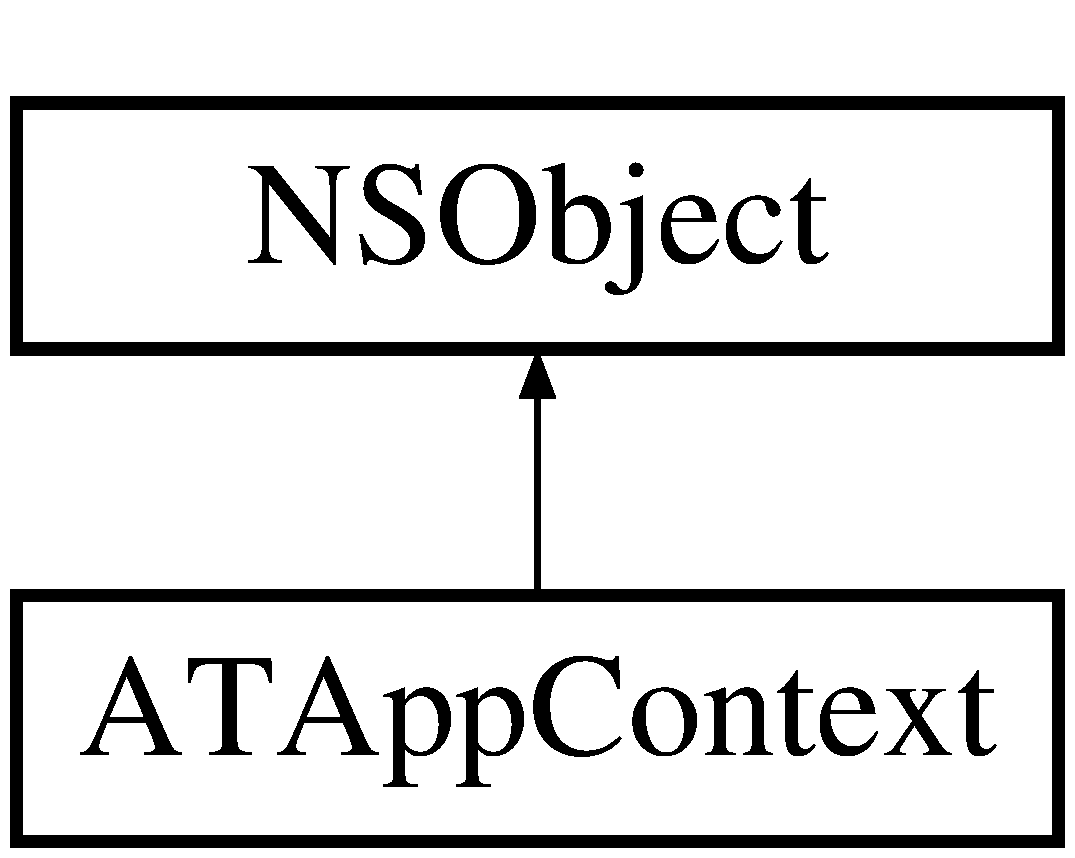
\includegraphics[height=2.000000cm]{interface_a_t_app_context}
\end{center}
\end{figure}
\subsubsection*{Public Member Functions}
\begin{DoxyCompactItemize}
\item 
\hypertarget{interface_a_t_app_context_a7e4fa14a4fba295c242147d0833ebfed}{
(id) -\/ {\bfseries initWithSynchronizer:appContext:}}
\label{interface_a_t_app_context_a7e4fa14a4fba295c242147d0833ebfed}

\item 
\hypertarget{interface_a_t_app_context_a94a02a8d89c8ae918d7ddb36ba527b48}{
(\hyperlink{class_n_s_managed_object}{NSManagedObject} $\ast$) -\/ {\bfseries objectAtURI:}}
\label{interface_a_t_app_context_a94a02a8d89c8ae918d7ddb36ba527b48}

\item 
\hypertarget{interface_a_t_app_context_a21b9499e171d899e7aecb70b582182ba}{
(\hyperlink{class_n_s_managed_object}{NSManagedObject} $\ast$) -\/ {\bfseries createAppObjectAtURI:}}
\label{interface_a_t_app_context_a21b9499e171d899e7aecb70b582182ba}

\item 
\hypertarget{interface_a_t_app_context_a3df88879a1cacecd35a7bc674f8fe605}{
(Class) -\/ {\bfseries \_\-managedClassForURI:}}
\label{interface_a_t_app_context_a3df88879a1cacecd35a7bc674f8fe605}

\item 
\hypertarget{interface_a_t_app_context_af5b706906b12bbae130ba97a1fd4f233}{
(\hyperlink{struct___a_t_object_u_r_i}{ATObjectURI}) -\/ {\bfseries URIOfAppObject:}}
\label{interface_a_t_app_context_af5b706906b12bbae130ba97a1fd4f233}

\item 
\hypertarget{interface_a_t_app_context_a5467ab26d0768fda050e72b7267dd4f2}{
(void) -\/ {\bfseries changeIDTo:atURI:}}
\label{interface_a_t_app_context_a5467ab26d0768fda050e72b7267dd4f2}

\item 
\hypertarget{interface_a_t_app_context_ab4b436e64d15f8d25d3f186479e4cf7d}{
(void) -\/ {\bfseries updateAppObject:withDictionary:}}
\label{interface_a_t_app_context_ab4b436e64d15f8d25d3f186479e4cf7d}

\item 
\hypertarget{interface_a_t_app_context_a2b43c323a64dcef375733da94ee63fd2}{
(void) -\/ {\bfseries deleteAppObject:}}
\label{interface_a_t_app_context_a2b43c323a64dcef375733da94ee63fd2}

\item 
\hypertarget{interface_a_t_app_context_ad590a1e779fcebf73218573783425151}{
(void) -\/ {\bfseries \_\-resolveRelations:withDictionary:}}
\label{interface_a_t_app_context_ad590a1e779fcebf73218573783425151}

\item 
\hypertarget{interface_a_t_app_context_a544871bcc8c6974f3bdf0edce58b5468}{
(NSDictionary $\ast$) -\/ {\bfseries dataForObject:}}
\label{interface_a_t_app_context_a544871bcc8c6974f3bdf0edce58b5468}

\item 
\hypertarget{interface_a_t_app_context_ab14fb60385ad32a8a2e91fa185c1f7d4}{
(NSArray $\ast$) -\/ {\bfseries relationsForAppObject:}}
\label{interface_a_t_app_context_ab14fb60385ad32a8a2e91fa185c1f7d4}

\item 
\hypertarget{interface_a_t_app_context_a344bf2060f78ed0968a5cf22c76949d2}{
(BOOL) -\/ {\bfseries attributesChangedInAppObject:}}
\label{interface_a_t_app_context_a344bf2060f78ed0968a5cf22c76949d2}

\item 
\hypertarget{interface_a_t_app_context_aa6f9c0e4fd9b9d542eda09bfcc2c2f7a}{
(BOOL) -\/ {\bfseries hasChanges}}
\label{interface_a_t_app_context_aa6f9c0e4fd9b9d542eda09bfcc2c2f7a}

\item 
\hypertarget{interface_a_t_app_context_a00ba90e776e4df7fc7d9dc3c0137138e}{
(void) -\/ {\bfseries save}}
\label{interface_a_t_app_context_a00ba90e776e4df7fc7d9dc3c0137138e}

\item 
\hypertarget{interface_a_t_app_context_a05e2eea400233f313641bd144109e1fb}{
(void) -\/ {\bfseries save:}}
\label{interface_a_t_app_context_a05e2eea400233f313641bd144109e1fb}

\item 
\hypertarget{interface_a_t_app_context_a05643fd02b9692dfaf1ebeea5bf84a6b}{
(void) -\/ {\bfseries obtainPermanentIDsForObjects:error:}}
\label{interface_a_t_app_context_a05643fd02b9692dfaf1ebeea5bf84a6b}

\end{DoxyCompactItemize}
\subsubsection*{Static Public Member Functions}
\begin{DoxyCompactItemize}
\item 
\hypertarget{interface_a_t_app_context_a00756fedbbc0ce79dd55c20862d47913}{
(id) + {\bfseries sharedAppContext}}
\label{interface_a_t_app_context_a00756fedbbc0ce79dd55c20862d47913}

\end{DoxyCompactItemize}
\subsubsection*{Protected Attributes}
\begin{DoxyCompactItemize}
\item 
\hypertarget{interface_a_t_app_context_af1c6f509bc2183767278e1e687ffcc0e}{
\hyperlink{interface_a_t_synchronizer}{ATSynchronizer} $\ast$ {\bfseries \_\-sync}}
\label{interface_a_t_app_context_af1c6f509bc2183767278e1e687ffcc0e}

\item 
\hypertarget{interface_a_t_app_context_ade3e164d9ec290b1b752f749c84a57c1}{
NSManagedObjectContext $\ast$ {\bfseries \_\-managedContext}}
\label{interface_a_t_app_context_ade3e164d9ec290b1b752f749c84a57c1}

\item 
\hypertarget{interface_a_t_app_context_addad5fb48d0bb32ca07a120bde680072}{
NSMutableArray $\ast$ {\bfseries \_\-relationsQueue}}
\label{interface_a_t_app_context_addad5fb48d0bb32ca07a120bde680072}

\end{DoxyCompactItemize}
\subsubsection*{Properties}
\begin{DoxyCompactItemize}
\item 
\hypertarget{interface_a_t_app_context_a9e4d6b12a7d2db4e642504ec45744a85}{
\hyperlink{interface_a_t_synchronizer}{ATSynchronizer} $\ast$ {\bfseries sync}}
\label{interface_a_t_app_context_a9e4d6b12a7d2db4e642504ec45744a85}

\item 
\hypertarget{interface_a_t_app_context_a38c53145eccd1f4fbbbea4a081dfd81e}{
NSManagedObjectContext $\ast$ {\bfseries managedContext}}
\label{interface_a_t_app_context_a38c53145eccd1f4fbbbea4a081dfd81e}

\item 
\hypertarget{interface_a_t_app_context_adc64825f25a7e7c6695ddcc8cc265822}{
\hyperlink{interface_a_t_attribute_mapper}{ATAttributeMapper} $\ast$ {\bfseries attributeMapper}}
\label{interface_a_t_app_context_adc64825f25a7e7c6695ddcc8cc265822}

\end{DoxyCompactItemize}


The documentation for this class was generated from the following files:\begin{DoxyCompactItemize}
\item 
ATAppContext.h\item 
ATAppContext.m\end{DoxyCompactItemize}

\hypertarget{interface_a_t_attribute_mapper}{
\subsubsection{ATAttributeMapper Class Reference}
\label{interface_a_t_attribute_mapper}\index{ATAttributeMapper@{ATAttributeMapper}}
}


{\ttfamily \#import $<$ATAttributeMapper.h$>$}

Inheritance diagram for ATAttributeMapper:\begin{figure}[h]
\begin{center}
\leavevmode
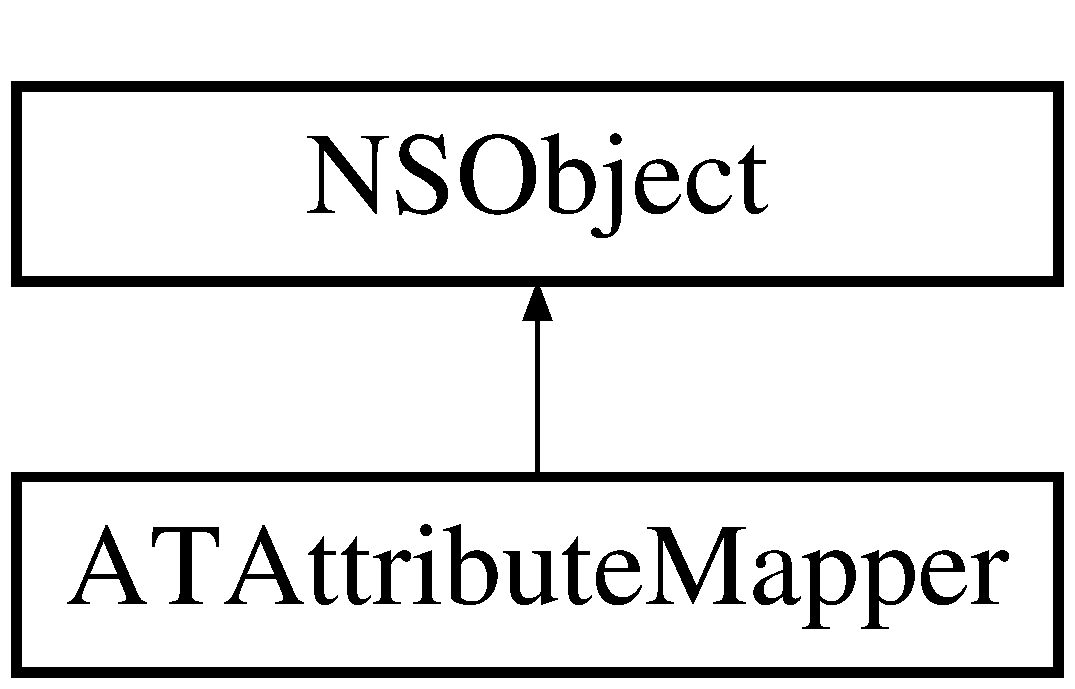
\includegraphics[height=2.000000cm]{interface_a_t_attribute_mapper}
\end{center}
\end{figure}
\subsubsection*{Public Member Functions}
\begin{DoxyCompactItemize}
\item 
\hypertarget{interface_a_t_attribute_mapper_ae1724904b0f49669626c87f07b4e0fd2}{
(id) -\/ {\bfseries initWithMappingHelper:}}
\label{interface_a_t_attribute_mapper_ae1724904b0f49669626c87f07b4e0fd2}

\end{DoxyCompactItemize}
\subsubsection*{Properties}
\begin{DoxyCompactItemize}
\item 
\hypertarget{interface_a_t_attribute_mapper_a2b8e7175248e56bbe8cd2217e23e9220}{
\hyperlink{interface_a_t_mapping_helper}{ATMappingHelper} $\ast$ {\bfseries mappingHelper}}
\label{interface_a_t_attribute_mapper_a2b8e7175248e56bbe8cd2217e23e9220}

\end{DoxyCompactItemize}


\subsubsection{Detailed Description}
This class does nothing 

The documentation for this class was generated from the following files:\begin{DoxyCompactItemize}
\item 
ATAttributeMapper.h\item 
ATAttributeMapper.m\end{DoxyCompactItemize}

\hypertarget{interface_a_t_connection_guard}{
\subsubsection{ATConnectionGuard Class Reference}
\label{interface_a_t_connection_guard}\index{ATConnectionGuard@{ATConnectionGuard}}
}
Inheritance diagram for ATConnectionGuard:\begin{figure}[h]
\begin{center}
\leavevmode
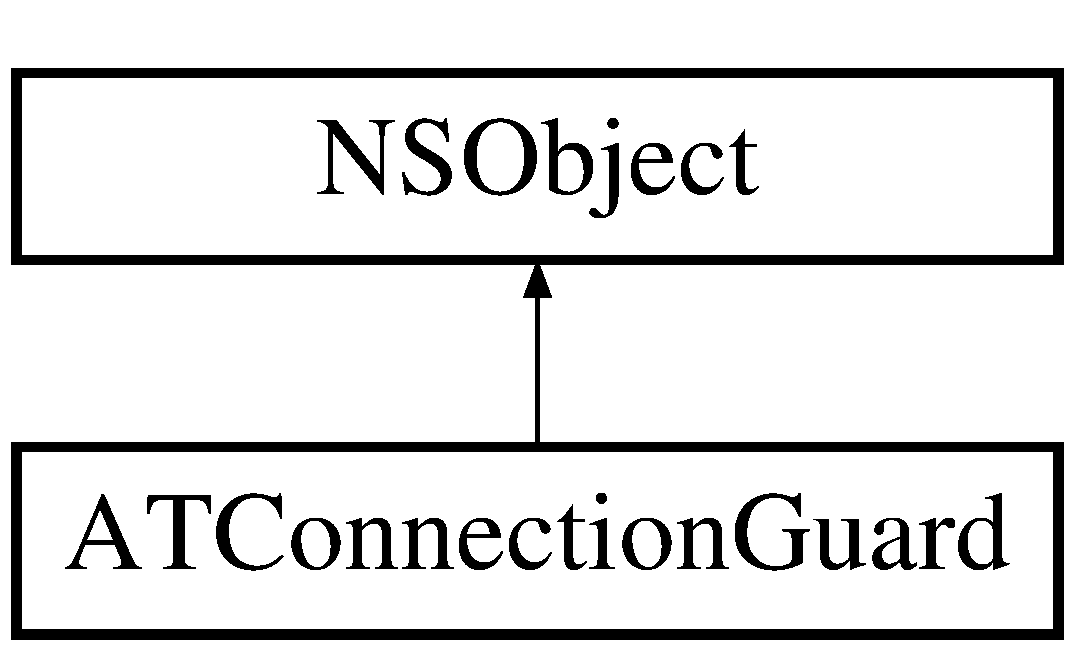
\includegraphics[height=2.000000cm]{interface_a_t_connection_guard}
\end{center}
\end{figure}
\subsubsection*{Public Member Functions}
\begin{DoxyCompactItemize}
\item 
\hypertarget{interface_a_t_connection_guard_a96b67e50d661e8e0edf6dd280dd03a7d}{
(void) -\/ {\bfseries start}}
\label{interface_a_t_connection_guard_a96b67e50d661e8e0edf6dd280dd03a7d}

\item 
\hypertarget{interface_a_t_connection_guard_a690563a6d28297f42209c29e016a961b}{
(void) -\/ {\bfseries stop}}
\label{interface_a_t_connection_guard_a690563a6d28297f42209c29e016a961b}

\item 
\hypertarget{interface_a_t_connection_guard_adc0892e3439bd48580bc8171d3cd9c5c}{
(void) -\/ {\bfseries \_\-checkConnection}}
\label{interface_a_t_connection_guard_adc0892e3439bd48580bc8171d3cd9c5c}

\end{DoxyCompactItemize}
\subsubsection*{Protected Attributes}
\begin{DoxyCompactItemize}
\item 
\hypertarget{interface_a_t_connection_guard_af213d51050cb2c17a7f85715fa602323}{
BOOL {\bfseries isRunning}}
\label{interface_a_t_connection_guard_af213d51050cb2c17a7f85715fa602323}

\end{DoxyCompactItemize}
\subsubsection*{Properties}
\begin{DoxyCompactItemize}
\item 
\hypertarget{interface_a_t_connection_guard_a6cafd79831265da735d92cec478192a0}{
\hyperlink{interface_a_t_synchronizer}{ATSynchronizer} $\ast$ {\bfseries client}}
\label{interface_a_t_connection_guard_a6cafd79831265da735d92cec478192a0}

\end{DoxyCompactItemize}


The documentation for this class was generated from the following files:\begin{DoxyCompactItemize}
\item 
ATConnectionGuard.h\item 
ATConnectionGuard.m\end{DoxyCompactItemize}

\hypertarget{interface_a_t_entity_fetch_request}{
\subsubsection{ATEntityFetchRequest Class Reference}
\label{interface_a_t_entity_fetch_request}\index{ATEntityFetchRequest@{ATEntityFetchRequest}}
}
Inheritance diagram for ATEntityFetchRequest:\begin{figure}[h]
\begin{center}
\leavevmode
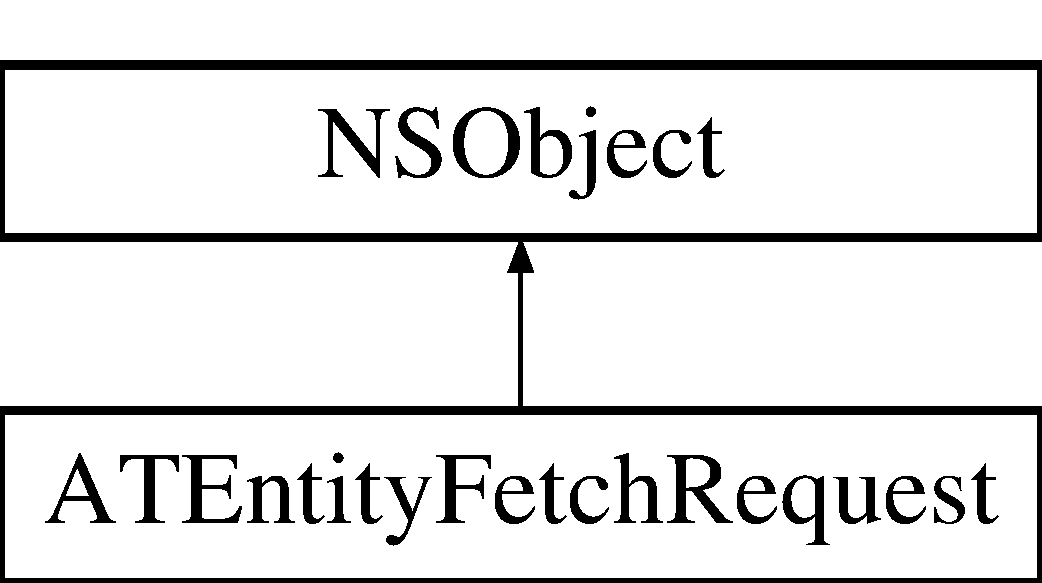
\includegraphics[height=2.000000cm]{interface_a_t_entity_fetch_request}
\end{center}
\end{figure}
\subsubsection*{Public Member Functions}
\begin{DoxyCompactItemize}
\item 
\hypertarget{interface_a_t_entity_fetch_request_a675e97f5dd42dc681c481648ef1d39b5}{
(id) -\/ {\bfseries initWithResourceClient:entity:}}
\label{interface_a_t_entity_fetch_request_a675e97f5dd42dc681c481648ef1d39b5}

\item 
\hypertarget{interface_a_t_entity_fetch_request_a72842e3aa37c2d86fb2f728aee1796fe}{
(void) -\/ {\bfseries send}}
\label{interface_a_t_entity_fetch_request_a72842e3aa37c2d86fb2f728aee1796fe}

\item 
\hypertarget{interface_a_t_entity_fetch_request_aef0c30154968bce6a9e0ead2c0c0fe98}{
(\hyperlink{struct___a_t_object_u_r_i}{ATObjectURI}) -\/ {\bfseries objectURIFromItem:}}
\label{interface_a_t_entity_fetch_request_aef0c30154968bce6a9e0ead2c0c0fe98}

\end{DoxyCompactItemize}
\subsubsection*{Properties}
\begin{DoxyCompactItemize}
\item 
\hypertarget{interface_a_t_entity_fetch_request_a187e3721b09b66577b6d2feba7ec0a4a}{
\hyperlink{interface_a_t_resource_client}{ATResourceClient} $\ast$ {\bfseries resourceClient}}
\label{interface_a_t_entity_fetch_request_a187e3721b09b66577b6d2feba7ec0a4a}

\item 
\hypertarget{interface_a_t_entity_fetch_request_ab59eb37b5bd6a386573c0ef591cad967}{
RKClient $\ast$ {\bfseries networkClient}}
\label{interface_a_t_entity_fetch_request_ab59eb37b5bd6a386573c0ef591cad967}

\item 
\hypertarget{interface_a_t_entity_fetch_request_afab560a9170c08b33c098f15b4399c01}{
\hyperlink{class_n_s_string}{NSString} $\ast$ {\bfseries entity}}
\label{interface_a_t_entity_fetch_request_afab560a9170c08b33c098f15b4399c01}

\end{DoxyCompactItemize}


The documentation for this class was generated from the following files:\begin{DoxyCompactItemize}
\item 
ATEntityFetchRequest.h\item 
ATEntityFetchRequest.m\end{DoxyCompactItemize}

\hypertarget{interface_a_t_mapping_helper}{
\subsubsection{ATMappingHelper Class Reference}
\label{interface_a_t_mapping_helper}\index{ATMappingHelper@{ATMappingHelper}}
}
Inheritance diagram for ATMappingHelper:\begin{figure}[h]
\begin{center}
\leavevmode
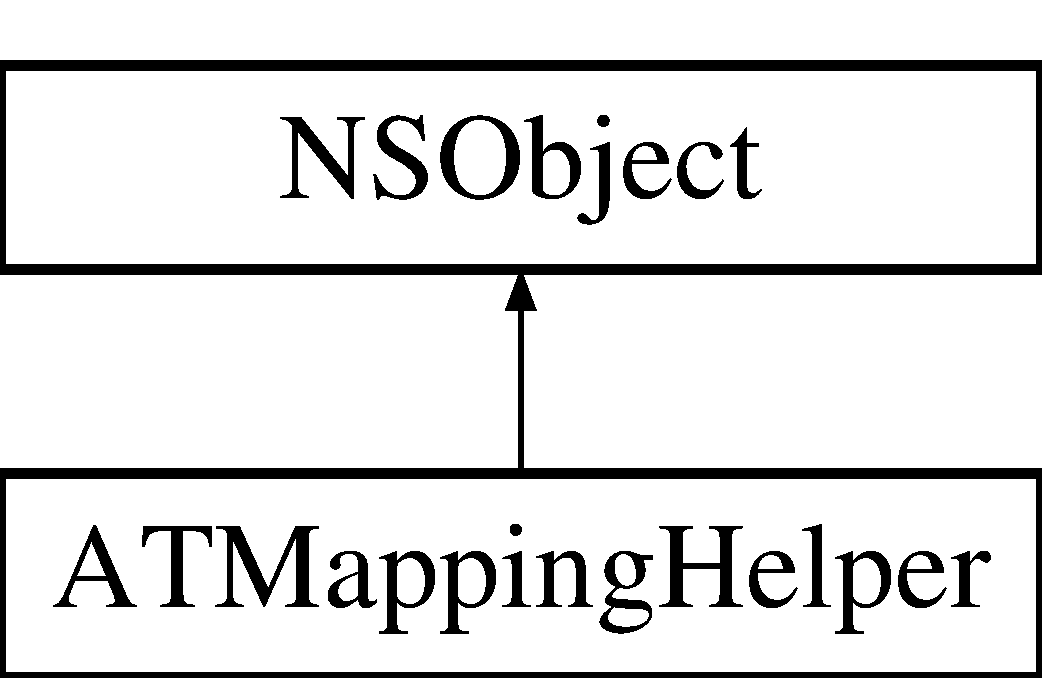
\includegraphics[height=2.000000cm]{interface_a_t_mapping_helper}
\end{center}
\end{figure}
\subsubsection*{Public Member Functions}
\begin{DoxyCompactItemize}
\item 
\hypertarget{interface_a_t_mapping_helper_a73fc4c531c66209f448ed0d79835fe56}{
(void) -\/ {\bfseries loadEntitiesMapFromResource:}}
\label{interface_a_t_mapping_helper_a73fc4c531c66209f448ed0d79835fe56}

\item 
\hypertarget{interface_a_t_mapping_helper_a9ec9ef5dc665692dce4fca0e6d050a0e}{
(void) -\/ {\bfseries loadAttributesMapFromResource:}}
\label{interface_a_t_mapping_helper_a9ec9ef5dc665692dce4fca0e6d050a0e}

\item 
\hypertarget{interface_a_t_mapping_helper_a9c616f062a025869711abbfe94796581}{
(void) -\/ {\bfseries loadRelationsMapFromResource:}}
\label{interface_a_t_mapping_helper_a9c616f062a025869711abbfe94796581}

\item 
\hypertarget{interface_a_t_mapping_helper_a0ab20c0f77c385dac21377dee445a3f6}{
(void) -\/ {\bfseries \_\-loadResource:intoDictionary:}}
\label{interface_a_t_mapping_helper_a0ab20c0f77c385dac21377dee445a3f6}

\item 
\hypertarget{interface_a_t_mapping_helper_a9fa5dd9036bd1e47208ca98a11003b2f}{
(\hyperlink{class_n_s_string}{NSString} $\ast$) -\/ {\bfseries localEntityNameFor:}}
\label{interface_a_t_mapping_helper_a9fa5dd9036bd1e47208ca98a11003b2f}

\item 
\hypertarget{interface_a_t_mapping_helper_aea4cc83c108b4dce637d7188b2015e5d}{
(\hyperlink{class_n_s_string}{NSString} $\ast$) -\/ {\bfseries serverEntityNameFor:}}
\label{interface_a_t_mapping_helper_aea4cc83c108b4dce637d7188b2015e5d}

\item 
\hypertarget{interface_a_t_mapping_helper_a339e9e1ee190e95be0c00cc86dc3794c}{
(\hyperlink{class_n_s_string}{NSString} $\ast$) -\/ {\bfseries serverEntityNameForAppObject:}}
\label{interface_a_t_mapping_helper_a339e9e1ee190e95be0c00cc86dc3794c}

\item 
\hypertarget{interface_a_t_mapping_helper_a045ecbcd62366a3de84fccc190bc7697}{
(\hyperlink{class_n_s_string}{NSString} $\ast$) -\/ {\bfseries serverAttributeNameFor:entity:}}
\label{interface_a_t_mapping_helper_a045ecbcd62366a3de84fccc190bc7697}

\item 
\hypertarget{interface_a_t_mapping_helper_a6096407dd2fee1da8af9a7dfc3256219}{
(\hyperlink{class_n_s_string}{NSString} $\ast$) -\/ {\bfseries localAttributeNameFor:entity:}}
\label{interface_a_t_mapping_helper_a6096407dd2fee1da8af9a7dfc3256219}

\item 
\hypertarget{interface_a_t_mapping_helper_af0532a90720b80d8c68f569cbef709c2}{
(NSDictionary $\ast$) -\/ {\bfseries relationsForObject:}}
\label{interface_a_t_mapping_helper_af0532a90720b80d8c68f569cbef709c2}

\item 
\hypertarget{interface_a_t_mapping_helper_aebeeba57781626e2ce67e7cdc695ba41}{
(NSDictionary $\ast$) -\/ {\bfseries relationsForEntity:}}
\label{interface_a_t_mapping_helper_aebeeba57781626e2ce67e7cdc695ba41}

\end{DoxyCompactItemize}
\subsubsection*{Properties}
\begin{DoxyCompactItemize}
\item 
NSDictionary $\ast$ \hyperlink{interface_a_t_mapping_helper_af42b5b8a8f037917548813611383da0f}{entitiesMap}
\item 
\hypertarget{interface_a_t_mapping_helper_abd9d756b7b5ed7a788ffcd9d1c8acc5c}{
NSDictionary $\ast$ {\bfseries attributesMap}}
\label{interface_a_t_mapping_helper_abd9d756b7b5ed7a788ffcd9d1c8acc5c}

\item 
\hypertarget{interface_a_t_mapping_helper_a9545ea64a1c4a6564aba6d30155fd47f}{
NSDictionary $\ast$ {\bfseries relationsMap}}
\label{interface_a_t_mapping_helper_a9545ea64a1c4a6564aba6d30155fd47f}

\end{DoxyCompactItemize}


\subsubsection{Property Documentation}
\hypertarget{interface_a_t_mapping_helper_af42b5b8a8f037917548813611383da0f}{
\index{ATMappingHelper@{ATMappingHelper}!entitiesMap@{entitiesMap}}
\index{entitiesMap@{entitiesMap}!ATMappingHelper@{ATMappingHelper}}
\subsubsection[{entitiesMap}]{\setlength{\rightskip}{0pt plus 5cm}-\/ (NSDictionary$\ast$) entitiesMap\hspace{0.3cm}{\ttfamily  \mbox{[}read, write, retain\mbox{]}}}}
\label{interface_a_t_mapping_helper_af42b5b8a8f037917548813611383da0f}
Entities map dictionary. Key represents server entity name and value represents client entity name 

The documentation for this class was generated from the following files:\begin{DoxyCompactItemize}
\item 
ATMappingHelper.h\item 
ATMappingHelper.m\end{DoxyCompactItemize}

\hypertarget{interface_a_t_message}{
\subsubsection{ATMessage Class Reference}
\label{interface_a_t_message}\index{ATMessage@{ATMessage}}
}
Inheritance diagram for ATMessage:\begin{figure}[h]
\begin{center}
\leavevmode
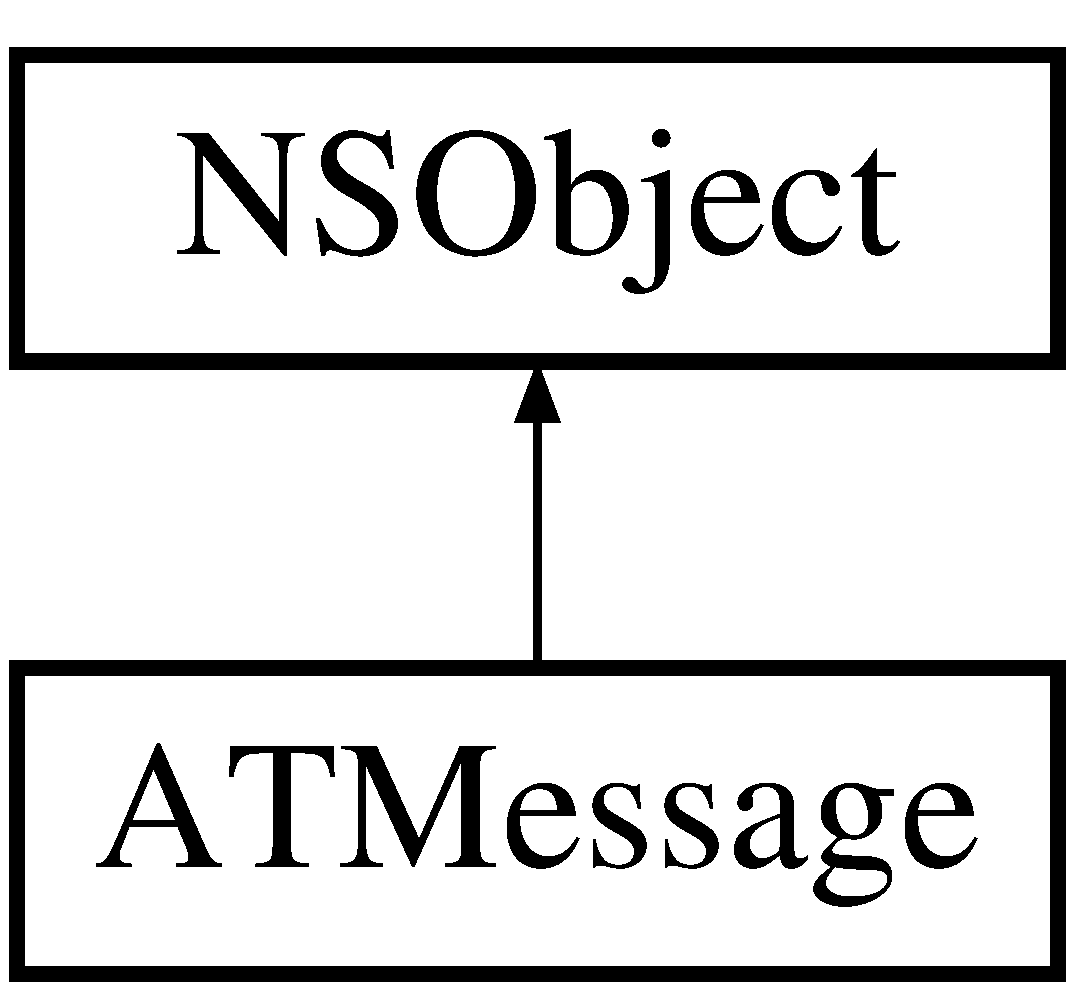
\includegraphics[height=2.000000cm]{interface_a_t_message}
\end{center}
\end{figure}
\subsubsection*{Public Member Functions}
\begin{DoxyCompactItemize}
\item 
\hypertarget{interface_a_t_message_a479b92f064ea3982fe3fa1dc0046da64}{
(\hyperlink{class_n_s_string}{NSString} $\ast$) -\/ {\bfseries JSONString}}
\label{interface_a_t_message_a479b92f064ea3982fe3fa1dc0046da64}

\end{DoxyCompactItemize}
\subsubsection*{Static Public Member Functions}
\begin{DoxyCompactItemize}
\item 
\hypertarget{interface_a_t_message_a899be809d07eddd49c7a69edcdbbc643}{
(\hyperlink{interface_a_t_message}{ATMessage} $\ast$) + {\bfseries messageFromJSONString:}}
\label{interface_a_t_message_a899be809d07eddd49c7a69edcdbbc643}

\end{DoxyCompactItemize}
\subsubsection*{Protected Attributes}
\begin{DoxyCompactItemize}
\item 
\hypertarget{interface_a_t_message_a55260e89bdf6b62ed070c9c3109e1717}{
\hyperlink{class_n_s_string}{NSString} $\ast$ {\bfseries \_\-type}}
\label{interface_a_t_message_a55260e89bdf6b62ed070c9c3109e1717}

\item 
\hypertarget{interface_a_t_message_adfc3efefff0092008dfc5a77ab28f093}{
NSDictionary $\ast$ {\bfseries \_\-content}}
\label{interface_a_t_message_adfc3efefff0092008dfc5a77ab28f093}

\end{DoxyCompactItemize}
\subsubsection*{Properties}
\begin{DoxyCompactItemize}
\item 
\hypertarget{interface_a_t_message_ae76aa0e54d3ec8380ba8b7d8fbcf7d9f}{
\hyperlink{class_n_s_string}{NSString} $\ast$ {\bfseries type}}
\label{interface_a_t_message_ae76aa0e54d3ec8380ba8b7d8fbcf7d9f}

\item 
\hypertarget{interface_a_t_message_a42e10d45f4235440c77a217bd6fcb2a8}{
NSDictionary $\ast$ {\bfseries content}}
\label{interface_a_t_message_a42e10d45f4235440c77a217bd6fcb2a8}

\end{DoxyCompactItemize}


The documentation for this class was generated from the following files:\begin{DoxyCompactItemize}
\item 
ATMessage.h\item 
ATMessage.m\end{DoxyCompactItemize}

\hypertarget{interface_a_t_message_client}{
\subsubsection{ATMessageClient Class Reference}
\label{interface_a_t_message_client}\index{ATMessageClient@{ATMessageClient}}
}


{\ttfamily \#import $<$ATMessageClient.h$>$}

Inheritance diagram for ATMessageClient:\begin{figure}[h]
\begin{center}
\leavevmode
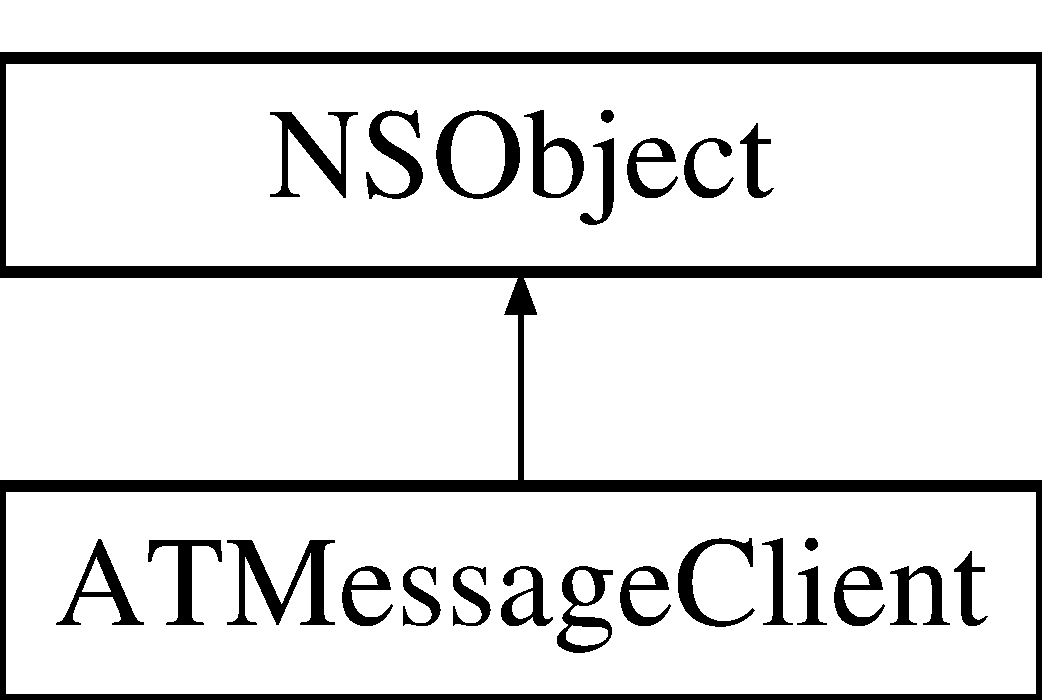
\includegraphics[height=2.000000cm]{interface_a_t_message_client}
\end{center}
\end{figure}
\subsubsection*{Public Member Functions}
\begin{DoxyCompactItemize}
\item 
\hypertarget{interface_a_t_message_client_ac3819bad54449ea9f46b3d9929bbf435}{
(id) -\/ {\bfseries initWithSynchronizer:}}
\label{interface_a_t_message_client_ac3819bad54449ea9f46b3d9929bbf435}

\item 
\hypertarget{interface_a_t_message_client_a5dc5708c4e13d7a75f78050b5f15249c}{
(void) -\/ {\bfseries connect}}
\label{interface_a_t_message_client_a5dc5708c4e13d7a75f78050b5f15249c}

\item 
\hypertarget{interface_a_t_message_client_ade89bb992bb85887edb8c22f877315e3}{
(BOOL) -\/ {\bfseries isConnected}}
\label{interface_a_t_message_client_ade89bb992bb85887edb8c22f877315e3}

\item 
\hypertarget{interface_a_t_message_client_aaf252625e14f5b125bc246eaa85a0c15}{
(void) -\/ {\bfseries \_\-initializeSocketConnection}}
\label{interface_a_t_message_client_aaf252625e14f5b125bc246eaa85a0c15}

\item 
\hypertarget{interface_a_t_message_client_ac73d19a7651d8e492c9ac97325640e0a}{
(void) -\/ {\bfseries \_\-sendConnectMessage}}
\label{interface_a_t_message_client_ac73d19a7651d8e492c9ac97325640e0a}

\item 
\hypertarget{interface_a_t_message_client_a79c2b59c186f18881680ab4fc1f277d1}{
(void) -\/ {\bfseries disconnect}}
\label{interface_a_t_message_client_a79c2b59c186f18881680ab4fc1f277d1}

\item 
\hypertarget{interface_a_t_message_client_a23c6f5dbb5a6358341d1707b91b86911}{
(void) -\/ {\bfseries \_\-didReceiveServerAuthFailure:}}
\label{interface_a_t_message_client_a23c6f5dbb5a6358341d1707b91b86911}

\item 
\hypertarget{interface_a_t_message_client_a2b1b29a59e25f19e2395b8cd51cf4c26}{
(void) -\/ {\bfseries \_\-didReceiveServerAuthSuccess:}}
\label{interface_a_t_message_client_a2b1b29a59e25f19e2395b8cd51cf4c26}

\item 
\hypertarget{interface_a_t_message_client_a03ec182577d528bc36c8999ea7e5b074}{
(void) -\/ {\bfseries sendMessage:}}
\label{interface_a_t_message_client_a03ec182577d528bc36c8999ea7e5b074}

\item 
\hypertarget{interface_a_t_message_client_a8e98344567ab31d6976978d5ccc172bd}{
(void) -\/ {\bfseries \_\-didReceiveServerPush:}}
\label{interface_a_t_message_client_a8e98344567ab31d6976978d5ccc172bd}

\end{DoxyCompactItemize}
\subsubsection*{Protected Attributes}
\begin{DoxyCompactItemize}
\item 
\hypertarget{interface_a_t_message_client_a59f618866758b87a03b2814d597ea143}{
BOOL {\bfseries \_\-isRunning}}
\label{interface_a_t_message_client_a59f618866758b87a03b2814d597ea143}

\item 
\hypertarget{interface_a_t_message_client_acd349f1b49d1ce1f335c58816bb8219a}{
\hyperlink{interface_a_t_synchronizer}{ATSynchronizer} $\ast$ {\bfseries \_\-sync}}
\label{interface_a_t_message_client_acd349f1b49d1ce1f335c58816bb8219a}

\item 
\hyperlink{class_n_s_string}{NSString} $\ast$ \hyperlink{interface_a_t_message_client_a10e7fe2e07ea9c28ca3cc987f85bff10}{\_\-host}
\item 
\hypertarget{interface_a_t_message_client_a13e73da308c7e71f864516a7b818d06c}{
NSInteger {\bfseries \_\-port}}
\label{interface_a_t_message_client_a13e73da308c7e71f864516a7b818d06c}

\item 
\hypertarget{interface_a_t_message_client_ad7ddc109d962798a2e64d7ba292e19e4}{
SocketIO $\ast$ {\bfseries \_\-connection}}
\label{interface_a_t_message_client_ad7ddc109d962798a2e64d7ba292e19e4}

\end{DoxyCompactItemize}
\subsubsection*{Properties}
\begin{DoxyCompactItemize}
\item 
\hypertarget{interface_a_t_message_client_a32d4d7b9e4f15f1595efca5ab85b1381}{
\hyperlink{interface_a_t_synchronizer}{ATSynchronizer} $\ast$ {\bfseries sync}}
\label{interface_a_t_message_client_a32d4d7b9e4f15f1595efca5ab85b1381}

\item 
\hypertarget{interface_a_t_message_client_a330b8c86d98c6ef9cbd8a8f3e2cae457}{
\hyperlink{class_n_s_string}{NSString} $\ast$ {\bfseries host}}
\label{interface_a_t_message_client_a330b8c86d98c6ef9cbd8a8f3e2cae457}

\item 
\hypertarget{interface_a_t_message_client_a8b889518a76ec8f627e401188761ebf1}{
NSInteger {\bfseries port}}
\label{interface_a_t_message_client_a8b889518a76ec8f627e401188761ebf1}

\item 
\hypertarget{interface_a_t_message_client_a301eb41f17a8ab3300e3d84b06ee8ceb}{
SocketIO $\ast$ {\bfseries connection}}
\label{interface_a_t_message_client_a301eb41f17a8ab3300e3d84b06ee8ceb}

\end{DoxyCompactItemize}


\subsubsection{Detailed Description}
\hyperlink{interface_a_t_message_client}{ATMessageClient} is responsible for dealing with live connection for push updates and notifications. 

\subsubsection{Member Data Documentation}
\hypertarget{interface_a_t_message_client_a10e7fe2e07ea9c28ca3cc987f85bff10}{
\index{ATMessageClient@{ATMessageClient}!\_\-host@{\_\-host}}
\index{\_\-host@{\_\-host}!ATMessageClient@{ATMessageClient}}
\subsubsection[{\_\-host}]{\setlength{\rightskip}{0pt plus 5cm}-\/ ({\bf NSString}$\ast$) {\bf \_\-host}\hspace{0.3cm}{\ttfamily  \mbox{[}protected\mbox{]}}}}
\label{interface_a_t_message_client_a10e7fe2e07ea9c28ca3cc987f85bff10}
Connection 

The documentation for this class was generated from the following files:\begin{DoxyCompactItemize}
\item 
ATMessageClient.h\item 
ATMessageClient.m\end{DoxyCompactItemize}

\hypertarget{interface_a_t_meta_context}{
\subsubsection{ATMetaContext Class Reference}
\label{interface_a_t_meta_context}\index{ATMetaContext@{ATMetaContext}}
}
Inheritance diagram for ATMetaContext:\begin{figure}[h]
\begin{center}
\leavevmode
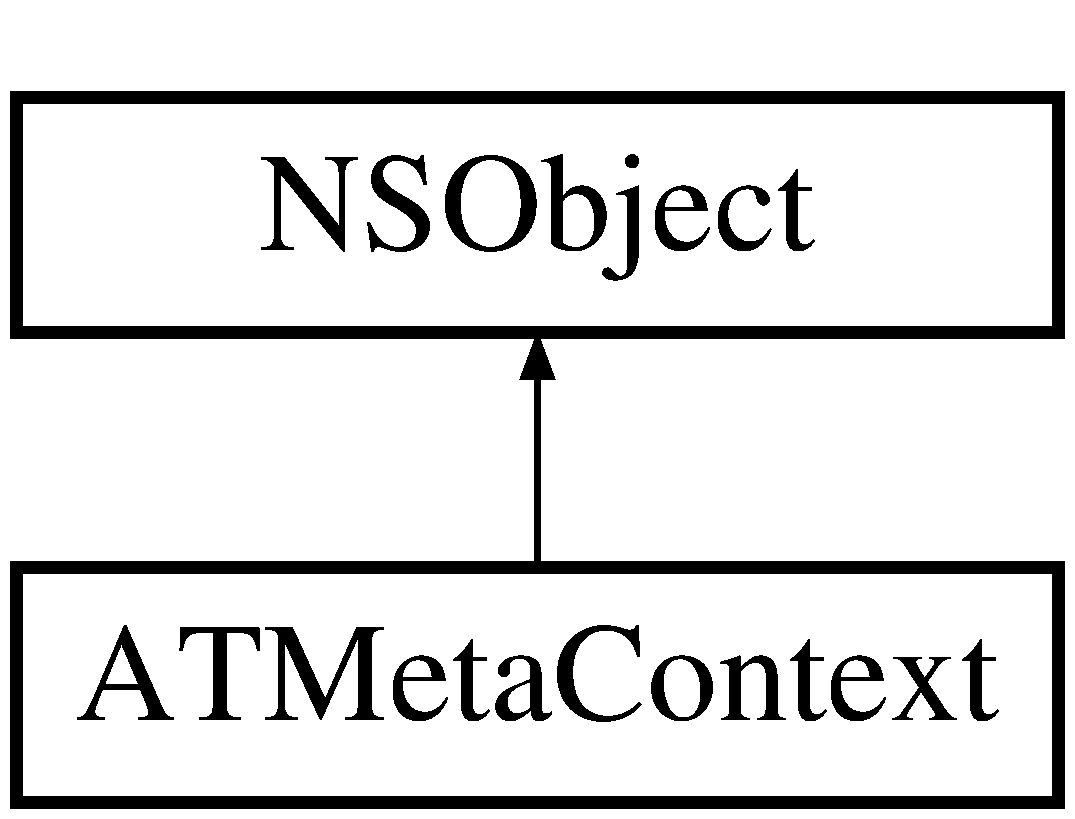
\includegraphics[height=2.000000cm]{interface_a_t_meta_context}
\end{center}
\end{figure}
\subsubsection*{Public Member Functions}
\begin{DoxyCompactItemize}
\item 
\hypertarget{interface_a_t_meta_context_adfa6a19a0196a1e47d82781f888c6136}{
(BOOL) -\/ {\bfseries save}}
\label{interface_a_t_meta_context_adfa6a19a0196a1e47d82781f888c6136}

\item 
\hypertarget{interface_a_t_meta_context_a374a353d6271cd493f9c5cf33630eb6b}{
(void) -\/ {\bfseries markURIChanged:}}
\label{interface_a_t_meta_context_a374a353d6271cd493f9c5cf33630eb6b}

\item 
\hypertarget{interface_a_t_meta_context_a6bcf5e7ee7c5b9a7c0fbccdf7723623c}{
(void) -\/ {\bfseries markURISynced:}}
\label{interface_a_t_meta_context_a6bcf5e7ee7c5b9a7c0fbccdf7723623c}

\item 
\hypertarget{interface_a_t_meta_context_a206094bc4db6c78668fb4593f0d59fec}{
(\hyperlink{interface_a_t_meta_object}{ATMetaObject} $\ast$) -\/ {\bfseries objectAtURI:}}
\label{interface_a_t_meta_context_a206094bc4db6c78668fb4593f0d59fec}

\item 
\hypertarget{interface_a_t_meta_context_a7b970df053c1bc1869ccb99945f383fb}{
(\hyperlink{interface_a_t_meta_object}{ATMetaObject} $\ast$) -\/ {\bfseries ensureObjectAtURI:}}
\label{interface_a_t_meta_context_a7b970df053c1bc1869ccb99945f383fb}

\item 
\hypertarget{interface_a_t_meta_context_af23b62b46612b08980a321f0b23cedd4}{
(\hyperlink{interface_a_t_meta_object}{ATMetaObject} $\ast$) -\/ {\bfseries createObjectAtURI:}}
\label{interface_a_t_meta_context_af23b62b46612b08980a321f0b23cedd4}

\item 
\hypertarget{interface_a_t_meta_context_a0cd0fe9a4ed8999db95f9bd843fb6536}{
(NSArray $\ast$) -\/ {\bfseries changedObjects}}
\label{interface_a_t_meta_context_a0cd0fe9a4ed8999db95f9bd843fb6536}

\item 
\hypertarget{interface_a_t_meta_context_a154ebbae634a69798821aa99f63e36f6}{
(void) -\/ {\bfseries changeIDTo:atURI:}}
\label{interface_a_t_meta_context_a154ebbae634a69798821aa99f63e36f6}

\end{DoxyCompactItemize}
\subsubsection*{Static Public Member Functions}
\begin{DoxyCompactItemize}
\item 
\hypertarget{interface_a_t_meta_context_a5ea6f84cd61278e7a69a5e466acb5ef6}{
(id) + {\bfseries restore}}
\label{interface_a_t_meta_context_a5ea6f84cd61278e7a69a5e466acb5ef6}

\item 
\hypertarget{interface_a_t_meta_context_aa958a238c2f8e661d92410aaa365af25}{
(\hyperlink{class_n_s_string}{NSString} $\ast$) + {\bfseries path}}
\label{interface_a_t_meta_context_aa958a238c2f8e661d92410aaa365af25}

\end{DoxyCompactItemize}
\subsubsection*{Protected Attributes}
\begin{DoxyCompactItemize}
\item 
\hypertarget{interface_a_t_meta_context_aa7bba9acdaedcefd8aeb096a36181a94}{
NSMutableDictionary $\ast$ {\bfseries \_\-objects}}
\label{interface_a_t_meta_context_aa7bba9acdaedcefd8aeb096a36181a94}

\end{DoxyCompactItemize}


The documentation for this class was generated from the following files:\begin{DoxyCompactItemize}
\item 
ATMetaContext.h\item 
ATMetaContext.m\end{DoxyCompactItemize}

\hypertarget{interface_a_t_meta_object}{
\subsubsection{ATMetaObject Class Reference}
\label{interface_a_t_meta_object}\index{ATMetaObject@{ATMetaObject}}
}
Inheritance diagram for ATMetaObject:\begin{figure}[h]
\begin{center}
\leavevmode
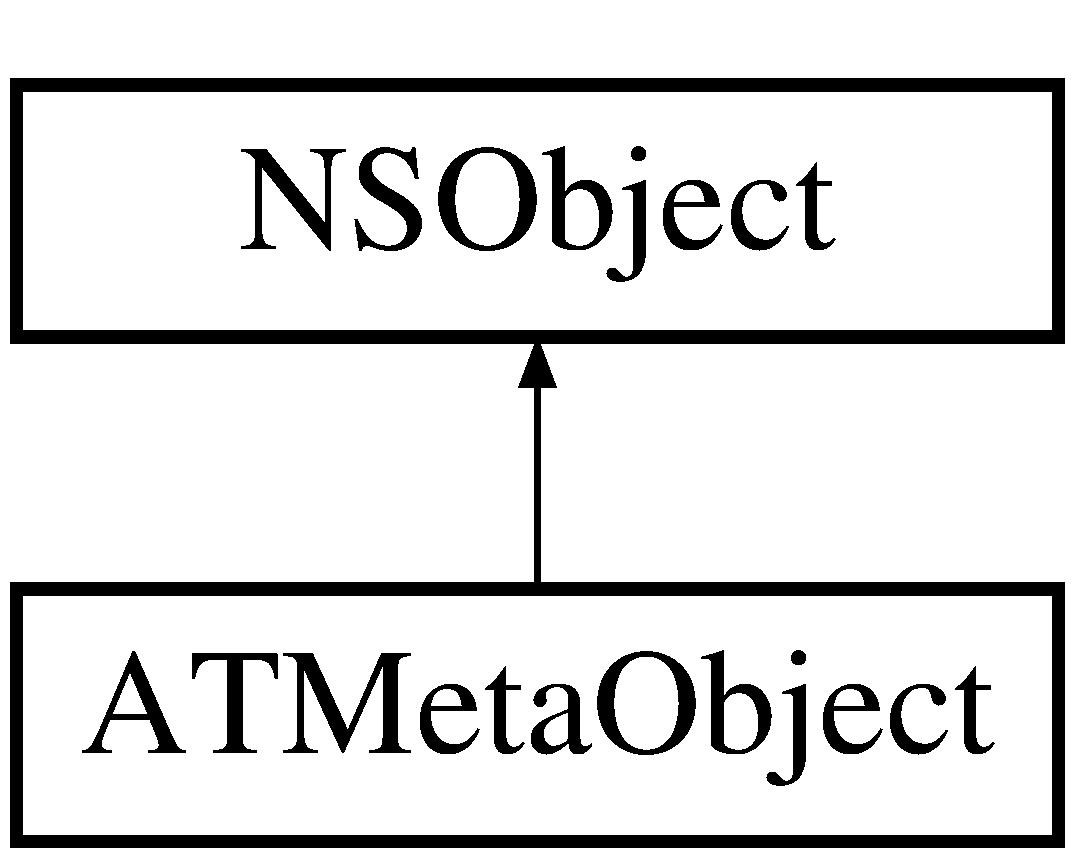
\includegraphics[height=2.000000cm]{interface_a_t_meta_object}
\end{center}
\end{figure}
\subsubsection*{Public Member Functions}
\begin{DoxyCompactItemize}
\item 
\hypertarget{interface_a_t_meta_object_afa20cebbc71d616926540f55230ed5ab}{
(id) -\/ {\bfseries initWithURI:}}
\label{interface_a_t_meta_object_afa20cebbc71d616926540f55230ed5ab}

\end{DoxyCompactItemize}
\subsubsection*{Properties}
\begin{DoxyCompactItemize}
\item 
\hypertarget{interface_a_t_meta_object_a7ecba236000b74241ae3931ccfc3e149}{
\hyperlink{struct___a_t_object_u_r_i}{ATObjectURI} {\bfseries uri}}
\label{interface_a_t_meta_object_a7ecba236000b74241ae3931ccfc3e149}

\item 
\hypertarget{interface_a_t_meta_object_a45ed797e32382c7b79b99aba02c83ed1}{
BOOL {\bfseries isChanged}}
\label{interface_a_t_meta_object_a45ed797e32382c7b79b99aba02c83ed1}

\item 
\hypertarget{interface_a_t_meta_object_ae63d1be418eb4fc20c2ac9e2996ad963}{
BOOL {\bfseries isLocalOnly}}
\label{interface_a_t_meta_object_ae63d1be418eb4fc20c2ac9e2996ad963}

\end{DoxyCompactItemize}


The documentation for this class was generated from the following files:\begin{DoxyCompactItemize}
\item 
ATMetaObject.h\item 
ATMetaObject.m\end{DoxyCompactItemize}

\hypertarget{interface_a_t_object_save_request}{
\subsubsection{ATObjectSaveRequest Class Reference}
\label{interface_a_t_object_save_request}\index{ATObjectSaveRequest@{ATObjectSaveRequest}}
}
Inheritance diagram for ATObjectSaveRequest:\begin{figure}[h]
\begin{center}
\leavevmode
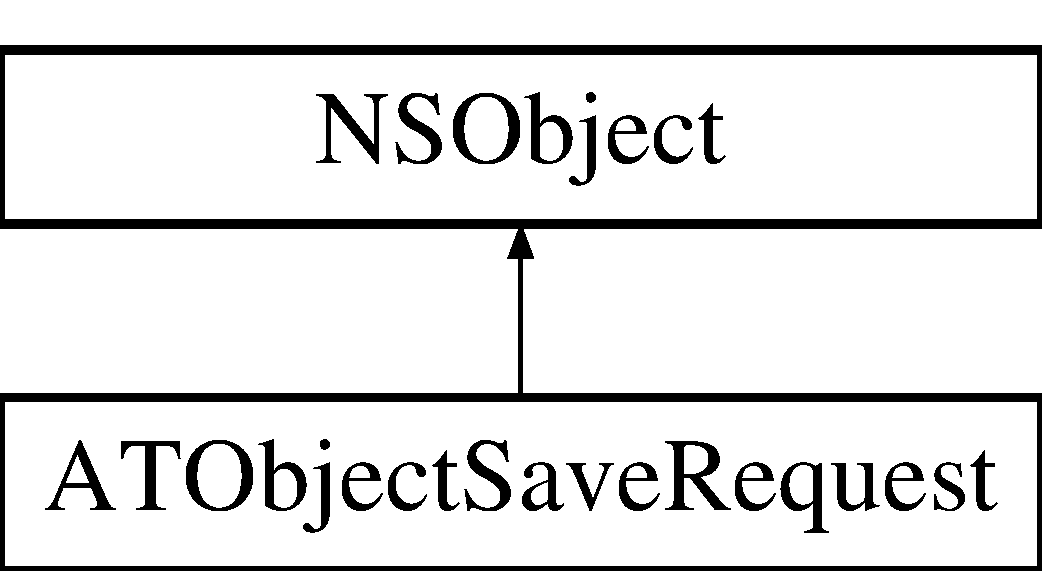
\includegraphics[height=2.000000cm]{interface_a_t_object_save_request}
\end{center}
\end{figure}
\subsubsection*{Public Member Functions}
\begin{DoxyCompactItemize}
\item 
\hypertarget{interface_a_t_object_save_request_a4251843e836ae9afa7b5ffb5e30bdb0f}{
(id) -\/ {\bfseries initWithResourceClient:object:options:}}
\label{interface_a_t_object_save_request_a4251843e836ae9afa7b5ffb5e30bdb0f}

\item 
\hypertarget{interface_a_t_object_save_request_a8bd540fab41eb1cbff19cba6519bf0f6}{
(void) -\/ {\bfseries send}}
\label{interface_a_t_object_save_request_a8bd540fab41eb1cbff19cba6519bf0f6}

\end{DoxyCompactItemize}
\subsubsection*{Properties}
\begin{DoxyCompactItemize}
\item 
\hypertarget{interface_a_t_object_save_request_a2d8d291a3e16bcea48ab0675b50e7cc6}{
\hyperlink{interface_a_t_resource_client}{ATResourceClient} $\ast$ {\bfseries resourceClient}}
\label{interface_a_t_object_save_request_a2d8d291a3e16bcea48ab0675b50e7cc6}

\item 
\hypertarget{interface_a_t_object_save_request_aec0386776e46384a4284711048edc747}{
RKClient $\ast$ {\bfseries networkClient}}
\label{interface_a_t_object_save_request_aec0386776e46384a4284711048edc747}

\item 
\hypertarget{interface_a_t_object_save_request_ac8448ee55f9108a6627ae8942be5ac84}{
NSDictionary $\ast$ {\bfseries options}}
\label{interface_a_t_object_save_request_ac8448ee55f9108a6627ae8942be5ac84}

\item 
\hypertarget{interface_a_t_object_save_request_a06cf1afe4dfd9bd6f851ed62175a4b2b}{
\hyperlink{class_n_s_managed_object}{NSManagedObject} $\ast$ {\bfseries object}}
\label{interface_a_t_object_save_request_a06cf1afe4dfd9bd6f851ed62175a4b2b}

\end{DoxyCompactItemize}


The documentation for this class was generated from the following files:\begin{DoxyCompactItemize}
\item 
ATObjectSaveRequest.h\item 
ATObjectSaveRequest.m\end{DoxyCompactItemize}

\hypertarget{interface_a_t_resource_client}{
\subsubsection{ATResourceClient Class Reference}
\label{interface_a_t_resource_client}\index{ATResourceClient@{ATResourceClient}}
}
Inheritance diagram for ATResourceClient:\begin{figure}[h]
\begin{center}
\leavevmode
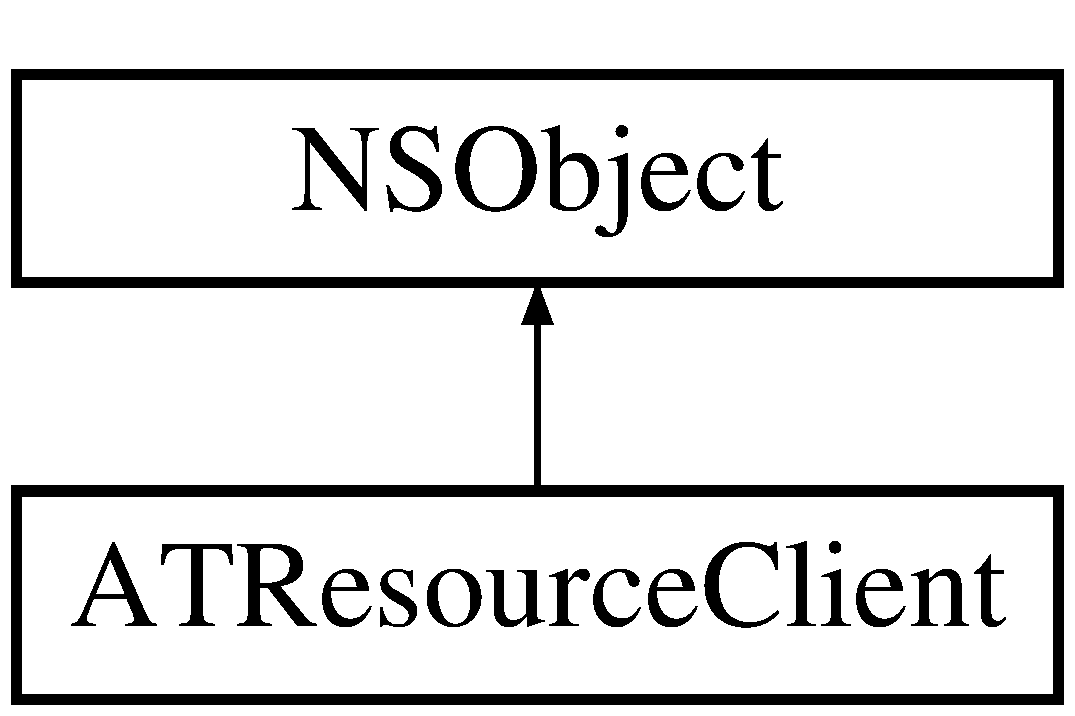
\includegraphics[height=2.000000cm]{interface_a_t_resource_client}
\end{center}
\end{figure}
\subsubsection*{Public Member Functions}
\begin{DoxyCompactItemize}
\item 
\hypertarget{interface_a_t_resource_client_a6a445159cd20e385d4088227ddbb5fa7}{
(id) -\/ {\bfseries initWithSynchronizer:}}
\label{interface_a_t_resource_client_a6a445159cd20e385d4088227ddbb5fa7}

\item 
\hypertarget{interface_a_t_resource_client_acc6bee940b9654a7625fd26f9dafc0a6}{
(void) -\/ {\bfseries setBaseURL:}}
\label{interface_a_t_resource_client_acc6bee940b9654a7625fd26f9dafc0a6}

\item 
\hypertarget{interface_a_t_resource_client_a5e92652d2cd5f04296272b9ef5a69aeb}{
(void) -\/ {\bfseries addHeader:withValue:}}
\label{interface_a_t_resource_client_a5e92652d2cd5f04296272b9ef5a69aeb}

\item 
\hypertarget{interface_a_t_resource_client_a71bad71ea56242fd19e5f48784689b5c}{
(void) -\/ {\bfseries fetchEntity:}}
\label{interface_a_t_resource_client_a71bad71ea56242fd19e5f48784689b5c}

\item 
\hypertarget{interface_a_t_resource_client_a53a5d620255bcc5dc198b4106f8141d3}{
(void) -\/ {\bfseries didFetchItem:withURI:}}
\label{interface_a_t_resource_client_a53a5d620255bcc5dc198b4106f8141d3}

\item 
\hypertarget{interface_a_t_resource_client_ac12de9fa49fa0340ac7f1d168214c986}{
(void) -\/ {\bfseries saveObject:}}
\label{interface_a_t_resource_client_ac12de9fa49fa0340ac7f1d168214c986}

\item 
\hypertarget{interface_a_t_resource_client_ac7150d971b28b7287523db7f29b76972}{
(void) -\/ {\bfseries saveObject:options:}}
\label{interface_a_t_resource_client_ac7150d971b28b7287523db7f29b76972}

\item 
\hypertarget{interface_a_t_resource_client_ae0201c8558a2e74caa524f0790c2bcef}{
(void) -\/ {\bfseries loadRoute:params:delegate:}}
\label{interface_a_t_resource_client_ae0201c8558a2e74caa524f0790c2bcef}

\item 
\hypertarget{interface_a_t_resource_client_aa9c928616e58786bdb15973e24fcd1af}{
(void) -\/ {\bfseries loadRoutesFromResource:}}
\label{interface_a_t_resource_client_aa9c928616e58786bdb15973e24fcd1af}

\item 
\hypertarget{interface_a_t_resource_client_a53ce9d8ae5a79f9a2f69cc861744109a}{
(\hyperlink{struct___a_t_route}{ATRoute}) -\/ {\bfseries routeForEntity:action:}}
\label{interface_a_t_resource_client_a53ce9d8ae5a79f9a2f69cc861744109a}

\item 
\hypertarget{interface_a_t_resource_client_aca4c252b5fc7af7ea5a41044665b6332}{
(\hyperlink{struct___a_t_route}{ATRoute}) -\/ {\bfseries routeForEntity:action:params:}}
\label{interface_a_t_resource_client_aca4c252b5fc7af7ea5a41044665b6332}

\end{DoxyCompactItemize}
\subsubsection*{Properties}
\begin{DoxyCompactItemize}
\item 
\hypertarget{interface_a_t_resource_client_a799228e0a82deb990c3fc58d69a212b3}{
\hyperlink{interface_a_t_synchronizer}{ATSynchronizer} $\ast$ {\bfseries sync}}
\label{interface_a_t_resource_client_a799228e0a82deb990c3fc58d69a212b3}

\item 
\hypertarget{interface_a_t_resource_client_afa980946f714b777325182bfa38da016}{
RKClient $\ast$ {\bfseries client}}
\label{interface_a_t_resource_client_afa980946f714b777325182bfa38da016}

\item 
\hypertarget{interface_a_t_resource_client_a12baa61aa58e54ccb95025ade33712d3}{
NSDictionary $\ast$ {\bfseries routes}}
\label{interface_a_t_resource_client_a12baa61aa58e54ccb95025ade33712d3}

\item 
\hypertarget{interface_a_t_resource_client_a47f4ef4c9464b546ba7b39eb212f2919}{
\hyperlink{class_n_s_string}{NSString} $\ast$ {\bfseries IDField}}
\label{interface_a_t_resource_client_a47f4ef4c9464b546ba7b39eb212f2919}

\end{DoxyCompactItemize}


The documentation for this class was generated from the following files:\begin{DoxyCompactItemize}
\item 
ATResourceClient.h\item 
ATResourceClient.m\end{DoxyCompactItemize}

\hypertarget{interface_a_t_synchronizer}{
\subsubsection{ATSynchronizer Class Reference}
\label{interface_a_t_synchronizer}\index{ATSynchronizer@{ATSynchronizer}}
}
Inheritance diagram for ATSynchronizer:\begin{figure}[h]
\begin{center}
\leavevmode
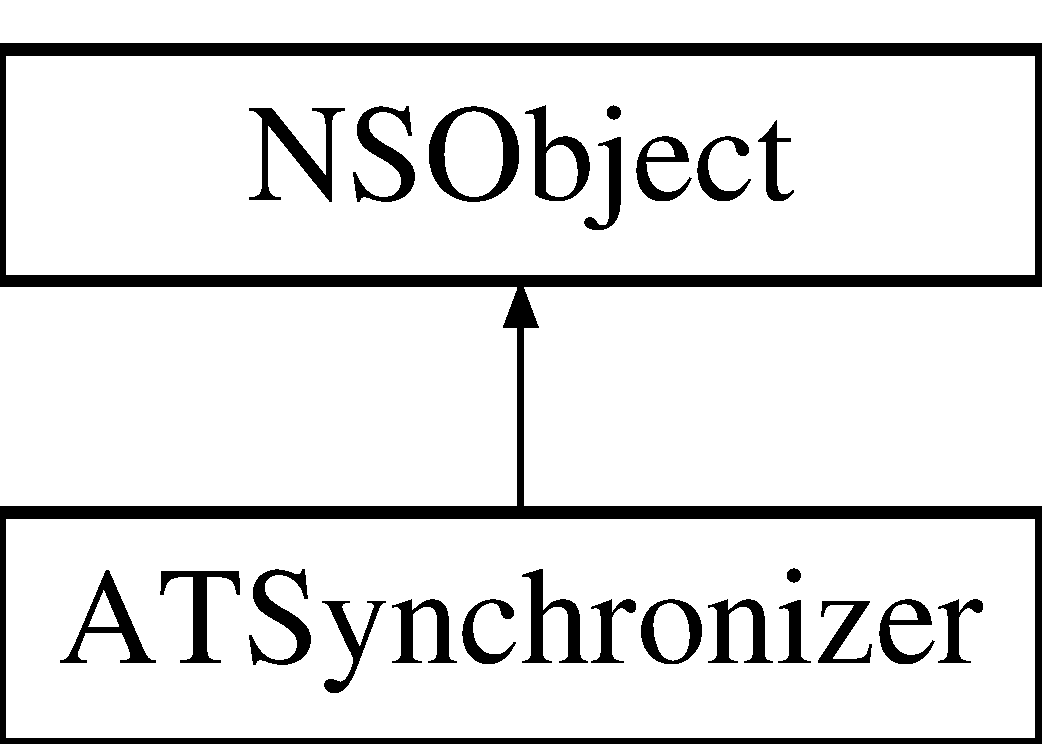
\includegraphics[height=2.000000cm]{interface_a_t_synchronizer}
\end{center}
\end{figure}
\subsubsection*{Public Member Functions}
\begin{DoxyCompactItemize}
\item 
\hypertarget{interface_a_t_synchronizer_a1a230c698ce38b033b22310db13120f5}{
(id) -\/ {\bfseries initWithAppContext:}}
\label{interface_a_t_synchronizer_a1a230c698ce38b033b22310db13120f5}

\item 
\hypertarget{interface_a_t_synchronizer_aa091026c249106b0f059a86ae9c5afd8}{
(void) -\/ {\bfseries close}}
\label{interface_a_t_synchronizer_aa091026c249106b0f059a86ae9c5afd8}

\item 
\hypertarget{interface_a_t_synchronizer_affb70ca203d9a187417db200776685c0}{
(\hyperlink{class_n_s_string}{NSString} $\ast$) -\/ {\bfseries authKeyOrNull}}
\label{interface_a_t_synchronizer_affb70ca203d9a187417db200776685c0}

\item 
\hypertarget{interface_a_t_synchronizer_a6b5f15941c11220049e877543e7adb62}{
(void) -\/ {\bfseries fetchEntity:}}
\label{interface_a_t_synchronizer_a6b5f15941c11220049e877543e7adb62}

\item 
\hypertarget{interface_a_t_synchronizer_ae7b25a346a2082dfbd5e54ac9ae6619f}{
(void) -\/ {\bfseries syncObject:}}
\label{interface_a_t_synchronizer_ae7b25a346a2082dfbd5e54ac9ae6619f}

\item 
\hypertarget{interface_a_t_synchronizer_adf5b437093a61f09ee914cc61e30f62d}{
(void) -\/ {\bfseries startSync}}
\label{interface_a_t_synchronizer_adf5b437093a61f09ee914cc61e30f62d}

\item 
\hypertarget{interface_a_t_synchronizer_add32dc8f725e3d33a8b49e9bea0460ba}{
(void) -\/ {\bfseries sync}}
\label{interface_a_t_synchronizer_add32dc8f725e3d33a8b49e9bea0460ba}

\item 
\hypertarget{interface_a_t_synchronizer_a063d9fcbbadfd834fded74a9a90de04e}{
(void) -\/ {\bfseries updateObjectAtURI:withDictionary:}}
\label{interface_a_t_synchronizer_a063d9fcbbadfd834fded74a9a90de04e}

\item 
\hypertarget{interface_a_t_synchronizer_a5975c374e80ef16d1131b8af6a3f1c17}{
(void) -\/ {\bfseries changeURIFrom:to:}}
\label{interface_a_t_synchronizer_a5975c374e80ef16d1131b8af6a3f1c17}

\item 
\hypertarget{interface_a_t_synchronizer_a237c7017d5b328901ef056c4174b1284}{
(void) -\/ {\bfseries startAutosync}}
\label{interface_a_t_synchronizer_a237c7017d5b328901ef056c4174b1284}

\item 
\hypertarget{interface_a_t_synchronizer_a50d1711cbe2f564ea1633e80fbc00dd7}{
(void) -\/ {\bfseries stopAutosync}}
\label{interface_a_t_synchronizer_a50d1711cbe2f564ea1633e80fbc00dd7}

\item 
\hypertarget{interface_a_t_synchronizer_a311d78f60c5b19b749bcc47ec43aa81b}{
(void) -\/ {\bfseries \_\-didChangeAppObject:}}
\label{interface_a_t_synchronizer_a311d78f60c5b19b749bcc47ec43aa81b}

\end{DoxyCompactItemize}
\subsubsection*{Protected Attributes}
\begin{DoxyCompactItemize}
\item 
\hyperlink{interface_a_t_mapping_helper}{ATMappingHelper} $\ast$ \hyperlink{interface_a_t_synchronizer_a31d09b73a13ca9815cd0f62d60dbc373}{\_\-mappingHelper}
\item 
\hyperlink{interface_a_t_meta_context}{ATMetaContext} $\ast$ \hyperlink{interface_a_t_synchronizer_a14e16b95fa385616596db1b540fb8280}{\_\-metaContext}
\item 
\hypertarget{interface_a_t_synchronizer_a4d68957b743ed4634a79496c9ce4857e}{
\hyperlink{interface_a_t_app_context}{ATAppContext} $\ast$ {\bfseries \_\-appContext}}
\label{interface_a_t_synchronizer_a4d68957b743ed4634a79496c9ce4857e}

\item 
\hyperlink{interface_a_t_message_client}{ATMessageClient} $\ast$ \hyperlink{interface_a_t_synchronizer_a7540768d28730fa0da9a29c8bd3db701}{\_\-messageClient}
\item 
\hypertarget{interface_a_t_synchronizer_ac8d7d4aca2cae90b6b218443d9dbcb77}{
\hyperlink{interface_a_t_resource_client}{ATResourceClient} $\ast$ {\bfseries \_\-resourceClient}}
\label{interface_a_t_synchronizer_ac8d7d4aca2cae90b6b218443d9dbcb77}

\item 
\hyperlink{class_n_s_string}{NSString} $\ast$ \hyperlink{interface_a_t_synchronizer_aff441de7abd4bb9fb6fb62ebfb36c072}{\_\-authKey}
\item 
\hypertarget{interface_a_t_synchronizer_a2f1074693dc133a3a76305842905cbe7}{
BOOL {\bfseries \_\-isSyncScheduled}}
\label{interface_a_t_synchronizer_a2f1074693dc133a3a76305842905cbe7}

\end{DoxyCompactItemize}
\subsubsection*{Properties}
\begin{DoxyCompactItemize}
\item 
\hypertarget{interface_a_t_synchronizer_aa4d38b9c8291f814c3e89a936e366748}{
\hyperlink{interface_a_t_meta_context}{ATMetaContext} $\ast$ {\bfseries metaContext}}
\label{interface_a_t_synchronizer_aa4d38b9c8291f814c3e89a936e366748}

\item 
\hypertarget{interface_a_t_synchronizer_ae4a168720bbd872e1fb509a951edc6f0}{
\hyperlink{interface_a_t_app_context}{ATAppContext} $\ast$ {\bfseries appContext}}
\label{interface_a_t_synchronizer_ae4a168720bbd872e1fb509a951edc6f0}

\item 
\hypertarget{interface_a_t_synchronizer_ad8ac915848318015ef77a42d367a4a64}{
\hyperlink{interface_a_t_mapping_helper}{ATMappingHelper} $\ast$ {\bfseries mappingHelper}}
\label{interface_a_t_synchronizer_ad8ac915848318015ef77a42d367a4a64}

\item 
\hypertarget{interface_a_t_synchronizer_a5506f23cbd14b9a27c6749a7eaf95d20}{
\hyperlink{interface_a_t_message_client}{ATMessageClient} $\ast$ {\bfseries messageClient}}
\label{interface_a_t_synchronizer_a5506f23cbd14b9a27c6749a7eaf95d20}

\item 
\hypertarget{interface_a_t_synchronizer_a11fbd96e8afa8f5a36c1be409d447053}{
\hyperlink{interface_a_t_resource_client}{ATResourceClient} $\ast$ {\bfseries resourceClient}}
\label{interface_a_t_synchronizer_a11fbd96e8afa8f5a36c1be409d447053}

\item 
\hypertarget{interface_a_t_synchronizer_aa10ad4a0dfe439088079385499f8e0ec}{
\hyperlink{class_n_s_string}{NSString} $\ast$ {\bfseries authKey}}
\label{interface_a_t_synchronizer_aa10ad4a0dfe439088079385499f8e0ec}

\item 
id$<$ \hyperlink{protocol_a_t_synchronizer_delegate-p}{ATSynchronizerDelegate} $>$ \hyperlink{interface_a_t_synchronizer_abef36e70ffe47396911ae10ed7c565a7}{delegate}
\end{DoxyCompactItemize}


\subsubsection{Member Data Documentation}
\hypertarget{interface_a_t_synchronizer_aff441de7abd4bb9fb6fb62ebfb36c072}{
\index{ATSynchronizer@{ATSynchronizer}!\_\-authKey@{\_\-authKey}}
\index{\_\-authKey@{\_\-authKey}!ATSynchronizer@{ATSynchronizer}}
\subsubsection[{\_\-authKey}]{\setlength{\rightskip}{0pt plus 5cm}-\/ ({\bf NSString}$\ast$) {\bf \_\-authKey}\hspace{0.3cm}{\ttfamily  \mbox{[}protected\mbox{]}}}}
\label{interface_a_t_synchronizer_aff441de7abd4bb9fb6fb62ebfb36c072}
State \hypertarget{interface_a_t_synchronizer_a31d09b73a13ca9815cd0f62d60dbc373}{
\index{ATSynchronizer@{ATSynchronizer}!\_\-mappingHelper@{\_\-mappingHelper}}
\index{\_\-mappingHelper@{\_\-mappingHelper}!ATSynchronizer@{ATSynchronizer}}
\subsubsection[{\_\-mappingHelper}]{\setlength{\rightskip}{0pt plus 5cm}-\/ ({\bf ATMappingHelper}$\ast$) {\bf \_\-mappingHelper}\hspace{0.3cm}{\ttfamily  \mbox{[}protected\mbox{]}}}}
\label{interface_a_t_synchronizer_a31d09b73a13ca9815cd0f62d60dbc373}
Helper \hypertarget{interface_a_t_synchronizer_a7540768d28730fa0da9a29c8bd3db701}{
\index{ATSynchronizer@{ATSynchronizer}!\_\-messageClient@{\_\-messageClient}}
\index{\_\-messageClient@{\_\-messageClient}!ATSynchronizer@{ATSynchronizer}}
\subsubsection[{\_\-messageClient}]{\setlength{\rightskip}{0pt plus 5cm}-\/ ({\bf ATMessageClient}$\ast$) {\bf \_\-messageClient}\hspace{0.3cm}{\ttfamily  \mbox{[}protected\mbox{]}}}}
\label{interface_a_t_synchronizer_a7540768d28730fa0da9a29c8bd3db701}
Networking clients \hypertarget{interface_a_t_synchronizer_a14e16b95fa385616596db1b540fb8280}{
\index{ATSynchronizer@{ATSynchronizer}!\_\-metaContext@{\_\-metaContext}}
\index{\_\-metaContext@{\_\-metaContext}!ATSynchronizer@{ATSynchronizer}}
\subsubsection[{\_\-metaContext}]{\setlength{\rightskip}{0pt plus 5cm}-\/ ({\bf ATMetaContext}$\ast$) {\bf \_\-metaContext}\hspace{0.3cm}{\ttfamily  \mbox{[}protected\mbox{]}}}}
\label{interface_a_t_synchronizer_a14e16b95fa385616596db1b540fb8280}
Context 

\subsubsection{Property Documentation}
\hypertarget{interface_a_t_synchronizer_abef36e70ffe47396911ae10ed7c565a7}{
\index{ATSynchronizer@{ATSynchronizer}!delegate@{delegate}}
\index{delegate@{delegate}!ATSynchronizer@{ATSynchronizer}}
\subsubsection[{delegate}]{\setlength{\rightskip}{0pt plus 5cm}-\/ (id$<$ {\bf ATSynchronizerDelegate} $>$) delegate\hspace{0.3cm}{\ttfamily  \mbox{[}read, write, assign\mbox{]}}}}
\label{interface_a_t_synchronizer_abef36e70ffe47396911ae10ed7c565a7}
Delegate 

The documentation for this class was generated from the following files:\begin{DoxyCompactItemize}
\item 
ATSynchronizer.h\item 
ATSynchronizer.m\end{DoxyCompactItemize}

\hypertarget{protocol_a_t_synchronizer_delegate-p}{
\subsubsection{$<$ATSynchronizerDelegate$>$ Protocol Reference}
\label{protocol_a_t_synchronizer_delegate-p}\index{ATSynchronizerDelegate-\/p@{ATSynchronizerDelegate-\/p}}
}
\subsubsection*{Public Member Functions}
\begin{DoxyCompactItemize}
\item 
\hypertarget{protocol_a_t_synchronizer_delegate-p_a5ef10b52a53f28e5f16cb76c2e9af9b8}{
(void) -\/ {\bfseries clientAuthDidSucceed:}}
\label{protocol_a_t_synchronizer_delegate-p_a5ef10b52a53f28e5f16cb76c2e9af9b8}

\item 
\hypertarget{protocol_a_t_synchronizer_delegate-p_a25d978a721f2bd286b9e063a1987f45d}{
(void) -\/ {\bfseries clientAuthDidFail:}}
\label{protocol_a_t_synchronizer_delegate-p_a25d978a721f2bd286b9e063a1987f45d}

\end{DoxyCompactItemize}
